\renewcommand{\thechapter}{}
\chapter{第一章~~绪论 (4学时)}
\renewcommand{\thechapter}{1}
\begin{itemize}
\item \textbf{主要内容}:
\item \textbf{重点和难点:}
\item \textbf{掌握:}
\item \textbf{理解:}
\item \textbf{了解:}
\end{itemize}

光学(optics)是一门有悠久历史的学科,它的发展史可追溯到2000多年前。如今,光学已是物理学最重要的一个分支. 主要经历以了下发展阶段.
\begin{itemize}
    \item 17世纪以前 光学知识和光学现象记录时代.
    \item 17世纪 W. 斯涅耳和R. 笛卡尔总结出光的反射定律和折射定律. 奠定了几何光学的基础, 光学真正形成一门学科. 
    \item 19世纪初,以杨氏干涉实验,惠更斯-菲涅耳原理和麦克斯韦方程为代表的波动光学建立
    \item 1900年,以普朗克能量子,爱因斯坦光量子,开启了量子光学的大门. 光学走向了量子时代 
    \item 1960年, 激光的发现和发展, 产生了一系列新的现化光学分支. 
\end{itemize}
  \begin{center}
       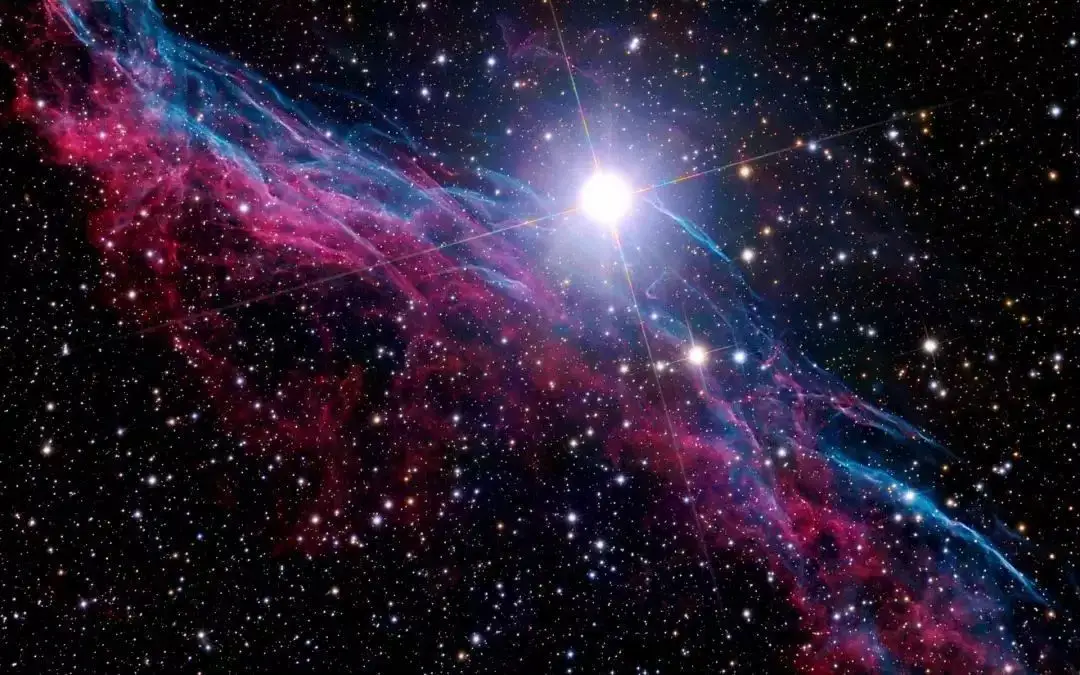
\includegraphics[width=0.6\textwidth]{figs/1.png}
  \end{center}

\section{光场的量子化}

\subsection{谐振子量子化}
1900年,普朗克在解释黑体辐射时,提出黑体由大量电谐振子构成, 电谐振子辐射量子化能量(光子),形成光场. \\ 
\subsubsection{经典解法}
谐振子在平衡位置附近的振动,在牛顿力学条件满足波动方程:
\begin{equation*}
    u_{tt}=a^2(u_{xx}+ u_{yy}+u_{zz})
\end{equation*}
零边界条件下的解(一维)
\begin{enumerate}
    \IItem 固有值:$\displaystyle  \lambda~_n=\frac{n^2\pi~^2}{l~^2}$ 
    \IItem 固有解:{\large $\displaystyle  X~_n(x)=\sin \frac{n\pi~}{l} x=\sin \omega_n x $}
    \IItem 基本解:
    \[u_n(x,t) = (a_n\cos\frac{ n\pi at}{l}+ b_n\sin \frac{ n\pi at}{l}) \sin \frac{ n\pi x}{l} \] 
    \IItem 叠加解:
    \[u(x,t) = \sum\limits_{n=1}^{\infty }  (a_n\cos\frac{ n\pi at}{l}+ b_n\sin \frac{ n\pi at}{l}) \sin \frac{ n\pi x}{l}\]
\end{enumerate}

\subsubsection{量子解法-1}
谐振子在平衡位置附近的振动, 写出其哈密顿量:
\[ H= T+V = \frac{p^2}{2m} +\frac{1}{2} m\omega ^2 x^2 \]

$x, p$ 是正则变量,有如下哈密顿正则方程
\[ \begin{aligned}
    \frac{\mathrm{d}p}{\mathrm{d}t} &= - \frac{\partial H}{\partial x} = - \omega ^2 x\\ 
    \frac{\mathrm{d}x}{\mathrm{d}t} &= \frac{\partial H}{\partial p} = \frac{p}{m}
  \end{aligned} \]

由基本对易关系
\[[\hat{x},\hat{p}]=i\hbar\]
得算符$\hat{p}=-i\hbar \frac{\partial }{\partial x}$
代回得量子化的哈密顿量  \[ H= -\frac{\hbar^2}{2m } \frac{d ^2}{x^2} + \frac{1}{2} m \omega ^2 x^2 \] 
代入薛定谔方程并求解 
\[i\hbar \frac{\partial }{\partial t} \Psi (x,t ) =H \Psi (x, t ) \]
得:
\begin{enumerate}
    \IItem 固有值:$\displaystyle  E_n=(n+\frac{1}{2})\hbar \omega $ 
    \IItem 固有函数:{$\displaystyle  X~_n(x)= H(\alpha x) e^{-(\alpha x)^2 /2 } $}
    \IItem 基本解:
    \[ \Psi_n(x,t) = N_n e^{-\frac{i}{\hbar} E_n t } X~_n(x)\]  
\end{enumerate}

\begin{remark}{正则量子化标准程序}
    \begin{itemize}
      \item 写出经典哈密顿
        \[E=H(x,p_x)\]
      \item 改写哈密顿为共轭变量形式$H(q,p)$, 并给出正则方程 
      \[ \begin{aligned}
        \frac{\mathrm{d}p}{\mathrm{d}t} &= - \frac{\partial H}{\partial q}  \\ 
        \frac{\mathrm{d}q}{\mathrm{d}t} &= \frac{\partial H}{\partial p} 
      \end{aligned} 
      \] 
      \item 共轭变量算符满足量子力学基本对易关系,得算符化哈密顿
       \[ [q,p] =i\hbar \]
      \item 把哈密顿算符代入薛定谔方程,得量子解. 
      \[i\hbar \frac{\partial }{\partial t} \rs{ \Psi}  =H \rs{ \Psi}   \]
    \end{itemize}
\end{remark}

\subsubsection{量子解法-2}
谐振子哈密顿量:
\[ H= \frac{p^2}{2m} +\frac{1}{2} m\omega ^2 x^2 \]
算符化哈密顿量
\[  \hat{H}= \frac{1}{2m} ({\hat{p}^2}+ m^2\omega ^2 \hat{x}^2 ) \qquad \text{with} \quad [\hat{x},\hat{p}]=i\hbar\]
薛定谔方程太难解! 有第二种解法. \\ 
令: 
\[ \hat{X} = \sqrt{\frac{m\omega}{\hbar}}\hat{x}, \hat{P} = \sqrt{\frac{1}{m \hbar \omega}} \hat{p} \]
重写哈密顿量
\[  \hat{H}= \frac{\hbar \omega }{2} (\hat{X}^2 + \hat{P}^2 ) \qquad \text{with} \quad [\hat{X},\hat{P}]=i \]
再令:
\[ \hat{a}= \frac{1 }{\sqrt{2}} (\hat{X} + i\hat{P} ), \qquad \hat{a}^\dagger= \frac{1 }{\sqrt{2}} (\hat{X} - i\hat{P} ) \]
重写哈密顿量
\[  \hat{H}= \hbar \omega \left(\hat{a}^\dagger \hat{a} + \frac{1 }{2}\right) \qquad \text{with} \quad [\hat{a},\hat{a}^\dagger]=1 \]
{\证} 为不失一般性,我们从正则变量进行证明, (在不影起混乱的条件,帽子可略去). \\
正则变量描述的密顿量
\[H= \frac{1}{2}(p ^2 + \omega ^2 q ^2) \]
重复上面的过程(取m=1),有:
\[\begin{aligned}
    a &= \frac{1}{\sqrt{2\hbar \omega}} (\omega q+i p)  \\ 
    a ^\dagger &= \frac{1}{\sqrt{2\hbar \omega}} (\omega q - i p)
\end{aligned}\]
    \[\begin{aligned}
        [a,a ^\dagger] &= a a ^\dagger- a ^\dagger a \\ 
        &= (\frac{1}{\sqrt{2\hbar \omega}})^2 [(\omega q+i p)(\omega q - i p)-(\omega q-i p)(\omega q + i p)] \\ 
        &= (\frac{1}{\sqrt{2\hbar \omega}})^2  2i\omega( p q - q  p) \\ 
        &= - (\frac{1}{\sqrt{2\hbar \omega}})^2  2i\omega[ q,  p]  \\
        &= - (\frac{1}{\sqrt{2\hbar \omega}})^2  2i\omega (i\hbar)  \\
        &= 1
    \end{aligned}\]
反向求得正则共轭变量算符的新形式
    \[ \begin{aligned}
      q &= \sqrt{\frac{\hbar}{2 \omega}} (a + a ^\dagger ) \\ 
      p &= i\sqrt{\frac{\hbar\omega}{2 }} (a^\dagger -a)  
    \end{aligned} 
    \] 
代入 $H= \frac{1}{2}(p ^2 + \omega ^2 q ^2 )$ \\ 
    \[ \begin{aligned}
        H& = \frac{1}{2} [ (i\sqrt{\frac{\hbar\omega}{2 }} (a^\dagger -a) )^2 + \omega ^2  (\sqrt{\frac{\hbar}{2 \omega}} (a + a ^\dagger ))^2] \\
        & = \frac{1}{2} [ (i\sqrt{\frac{\hbar\omega}{2 }} (a^\dagger -a) )^2 +  (\sqrt{\frac{\hbar\omega}{2 }} (a + a ^\dagger ))^2] \\
        & = \frac{1}{4}\hbar \omega [(a + a ^\dagger )^2-( a ^\dagger - a)^2 ] \\
        & = \frac{1}{4}\hbar \omega [2a a ^\dagger -  2a^\dagger a  + 4a ^\dagger a  ] \\
        &=  \hbar \omega (a ^\dagger a + \frac{1}{2})
      \end{aligned} 
      \] 
以上过程,同样适用于谐振子. \\ 

很明显, $ a \not =  a^\dagger $, 它不是自伴算符,不具厄密性. 有必要研究其具体性质.\\ 
对于能量第n个本征态,  
  \[ H  \rs{n} = E_n  \rs{n}, \quad  aH  \rs{n} =E_n a \rs{n}\]
  \[
  \begin{aligned}
        H a \rs{n} &= ( \hbar \omega a ^\dagger a + \frac{1}{2}\hbar \omega )a \rs{n} \\ 
        &=  ( \hbar \omega  a ^\dagger a a  + \frac{1}{2}\hbar \omega a ) \rs{n} \\ 
        &=  ( \hbar \omega  (-1+a a ^\dagger )a + \frac{1}{2}\hbar \omega a ) \rs{n} \\ 
        &=  ( \hbar \omega  a a ^\dagger a -  a \frac{1}{2}\hbar \omega ) \rs{n} \\ 
        &=  a( \hbar \omega   a ^\dagger a -  \frac{1}{2}\hbar \omega ) \rs{n} 
  \end{aligned}
  \]

  \[ 
  \begin{aligned}
    H a \rs{n}  &=  a( \hbar \omega   a ^\dagger a +  \frac{1}{2}\hbar \omega  - \hbar \omega ) \rs{n} \\ 
        &=  (aH - a \hbar \omega ) \rs{n} \\ 
        &=  (E_n -  \hbar \omega ) a\rs{n} \\ 
  \end{aligned}
  \]
  也就是说 $a \rs{n} $ 也是能量本征态, 本征值为 $E_n -  \hbar \omega = E_{n-1} $ 即有一份能量$ \hbar \omega $ 被湮灭, 故称 $a$ 为 湮灭算符, 有: 
  \[ \boxed{a \rs{n}= D_n\rs{n-1}} \]
同理可得: 
\[  H a^\dagger \rs{n}  =  (E_n +  \hbar \omega ) a^\dagger \rs{n} \]
也就是说 $a^\dagger\rs{n} $ 也是能量本性态, 本征值为 $E_n + \hbar \omega = E_{n+1} $ 即产生一份能量$ \hbar \omega $, 故称 $a^\dagger$ 为产生算符, 有: 
\[ \boxed{a^\dagger \rs{n}= C_n \rs{n+1}} \]

本征能量可无限地增加,但不能被无限湮灭,设最小的为$E_0$, 对应本征态$\rs{0}$, 有:
\[ \boxed{a \rs{0}= 0 }\]
~~\\ 
由 \[H=\hbar \omega a ^\dagger a + \frac{1}{2}\hbar \omega\]  
有: 
\[H-\frac{1}{2}\hbar \omega=\hbar \omega a ^\dagger a \] 
\[ 
\begin{aligned}
(H-\frac{1}{2}\hbar \omega) \rs{0} &= \hbar \omega a ^\dagger a \rs{0} = \hbar \omega a ^\dagger 0 = 0 \\ 
H \rs{0} &= \frac{1}{2}\hbar \omega \rs{0}=E_0 \rs{0} 
\end{aligned}
\] 
即, 谐振子的最低能级为
\[ \boxed{E_0=\dfrac{1}{2}\hbar \omega} \]
称为真空态.\\ 

从真空态出发, 相继使用产生算符,每次产生一份能量 $ \hbar \omega$, 因此谐振子的能量本征值为
\[\boxed{E_n = (n+\frac{1}{2})\hbar \omega, \qquad n=0,1,2, \cdots}  \] 
~~\\

\subsubsection{粒子数态}

对于黑体辐射场来说, 能量本征态$\rs{n}$描述的是该模($\omega$)上有$n$个激发的光子, 每个光子的能量都是 $\hbar \omega$ 即 :$\rs{n}$态描述的是含有$n$个光量子的态. 因此,能量本征态$\rs{n}$也称为粒子数态. \\ 

占有数算符是$ N=a^\dagger a $, 有本征方程:
\[ a^\dagger a \rs{n}= n\rs{n}\] 

产生湮灭算符分别产生和消灭这个模式的一个光子
\[ {a \rs{n}= D_n\rs{n-1}}, \qquad a^\dagger \rs{n}= C_n \rs{n+1} \]  
\[ 
  \begin{aligned}
    a^\dagger a \rs{n} &= a^\dagger D_n\rs{n-1} \\ 
    &= D_n C_{n-1} \rs{n} = n \rs{n} \\ 
    D_n C_{n-1}&=n \qquad \cdots (1)
  \end{aligned}
  \] 
  \[ 
    \begin{aligned}
      D_n &=  \lcr{n-1}{a}{n} \\
      &=  (\lcr{n}{a^\dagger }{n-1})^* \\
      &= C_{n-1} ^*   \qquad \cdots (2)
    \end{aligned}
    \] 
    联立(1)(2), 得 $C_{n-1}=\sqrt{n}= D_n, C_{n}=\sqrt{n+1} $\\ 

\subsection{单模光场的量子化}

\begin{center}
     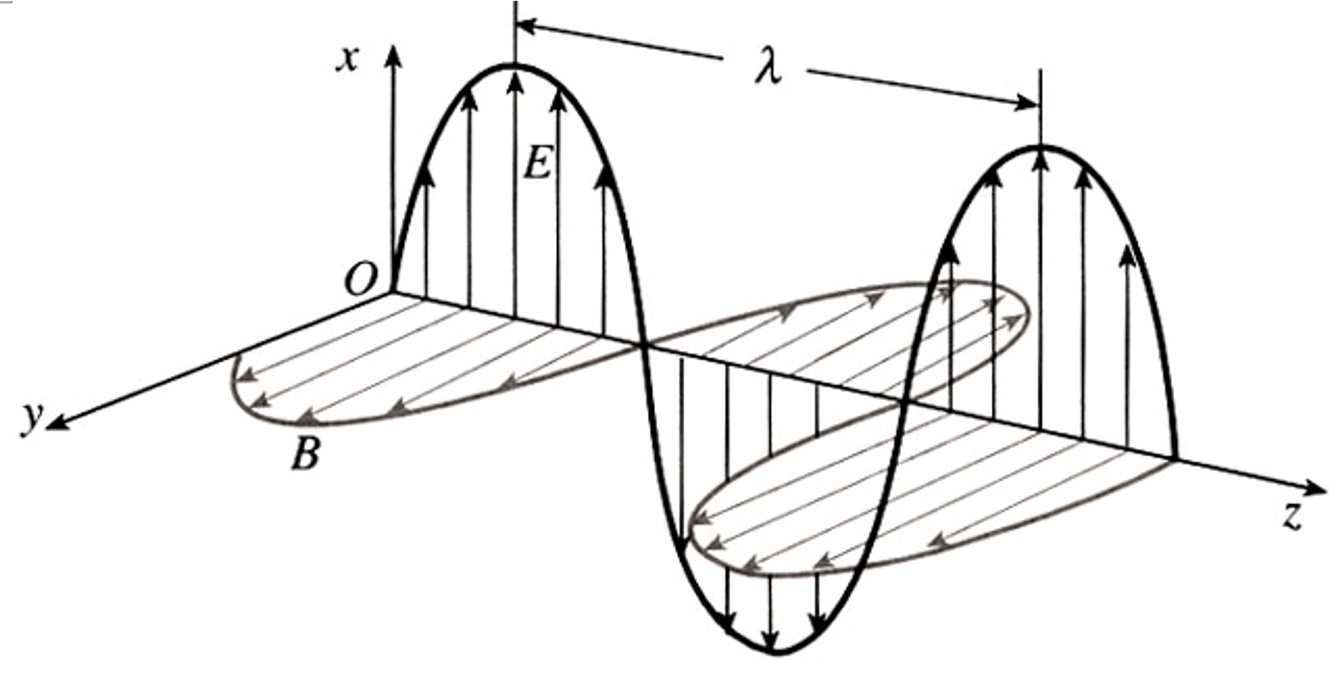
\includegraphics[width=0.55\textwidth]{figs/43.png}
\end{center}
考虑一个光学腔,其电磁场的能量密度 
\[ \omega = \frac{1}{2} (\epsilon_0 E^2 _x + \mu_0 H^2 _y) \]
总能量用哈密顿量描述
\[ H = \frac{1}{2} \int_V (\epsilon_0 E^2 _x + \mu_0 H^2 _y) dV \]

\subsubsection{经典解法}

介质中, 定义电位移矢量$\mathbf{D}$ 和 磁场强度 $\mathbf{H}$
\[ \mathbf{D}=\epsilon_0 \mathbf{E} + \mathbf{P} = \epsilon_0 \epsilon_r \mathbf{E},  \qquad \mathbf{H}=\frac{1}{\mu_0} \mathbf{B} -\mathbf{M}= \frac{1}{\mu_0\mu_r}\mathbf{B} \]
麦克斯韦方程:
\[ \begin{array}{l}  
  \nabla \cdot \mathbf{D} =\rho _f \\  
  \nabla \cdot \mathbf{B} = 0 \\  
  \nabla \times  \mathbf{E} = -\cfrac{\partial \mathbf{B}}{\partial t }  \\  
  \nabla \times  \mathbf{H} = \mathbf{J}_f +  \cfrac{\partial \mathbf{D}}{\partial t }   
\end{array} \]

对于真空 ($\rho _f =0, \mathbf{J}_f =0 $), 把 \[ \mathbf{B} = \mu_0 \mathbf{H}, \qquad  \mathbf{D} = \epsilon_0 \epsilon_r \mathbf{E} \]
代入如下麦克斯韦方程
 \[ \nabla \times  \mathbf{H} = \mathbf{J}_f +  \cfrac{\partial \mathbf{D}}{\partial t } \]
得: \[ \nabla \times \mathbf{B} = \mu_0\epsilon_0 \epsilon_r \cfrac{\partial \mathbf{E}} {\partial t } \]
\[
\begin{aligned}
  \nabla \times (\nabla \times  \mathbf{E}) &= - \nabla \times \cfrac{\partial \mathbf{B}}{\partial t } \\
  &= - \mu_0\epsilon_0 \epsilon_r \cfrac{\partial ^2 \mathbf{E}} {\partial t^2 }
\end{aligned} \]
由于
  \[
  \begin{aligned}
      \nabla \times (\nabla \times  \mathbf{E}) &=  \nabla (\nabla \cdot  \mathbf{E})- \nabla^2 \mathbf{E} \\
      &= - \nabla^2 \mathbf{E} 
  \end{aligned} \]
  得:
  \[
  \nabla^2 \mathbf{E}= \mu_0\epsilon_0 \epsilon_r \cfrac{\partial ^2 \mathbf{E}} {\partial t^2 }\]
  改写成
  \[\boxed{E_{tt} =c^2\nabla^2 \mathbf{E}}\]
  ~~\\
  这是波动方程的标准型(见数理方程) \\

  当电磁波在$z$方向传波时, 有$E_y=E_z=0, B_x=B_z=0$.\\ 
  考虑一个光学腔$0\leq z\leq L$, 其解为:
  \begin{enumerate}
    \IItem 固有值:$\displaystyle  \lambda_n=\frac{n^2\pi^2}{L^2}= k^2 _n $ 
    \IItem 固有解:$\displaystyle  E_n(z)=\sin (k_n z) $
    \IItem 基本解:$\displaystyle E_{x,n}(z,t) = a_n q_n (t) \sin (k_n z) $
    \IItem 叠加解:$\displaystyle E_{x}(z,t) = \sum\limits_{n=1}^{\infty } a_n q_n (t) \sin (k_n z)$
\end{enumerate}	
把解代入下式
\[ \nabla \times \mathbf{B} = \mu_0\epsilon_0 \epsilon_r \cfrac{\partial \mathbf{E}} {\partial t } \]
得磁场的解: 
\begin{enumerate}
  \IItem 叠加解:$\displaystyle H_{y}(z,t) = \sum\limits_{n=1}^{\infty } a_n \frac{\epsilon_0}{k_n}q_n ' (t) \cos (k_n z)$
\end{enumerate}	
经典结论: 电磁场的运动可分解为一系列基本模式的振动,在自由场条件下,振动是自由的,若有电荷或电流,变成受迫振动. \\


\subsubsection{量子化}

{\noindent \Bullet}现代物理学对场与粒子的关系有如下基本认识
\begin{enumerate}
    \item 场是物质存在的基本形式
    \item 所有的粒子都是场的量子,分为费米子和玻色子两大类
    \item 场的量子与量子力学中的粒子并不完全一样,在非相对论近似下两者可拟合在一起
    \item 光子无非相对论近似,不可能被拟合成量子力学中粒子的的样子
    \item 电磁场量子化有着不同于一般意义的效应.
\end{enumerate}

\subsubsection{简振模展开} 

注意光腔电磁波的叠加解(三维形式)
\[ \begin{aligned}
    \mathbf{E}( \mathbf{r},t) =& - \frac{1}{\sqrt{ \epsilon_0}} \sum_l ^\infty q_l(t) \mathbf{E}_l( \mathbf{r}) \\
    \mathbf{H}( \mathbf{r},t) =&  \frac{1}{\sqrt{ \mu_0}} \sum_l ^\infty \omega_l p_l(t) \mathbf{H}_l( \mathbf{r}) \\
 \end{aligned} 
\] 
是电磁场按腔模式的展开式, 解代入电磁场的哈密顿量,利用腔模正交性计算(细节!)
    \[ \begin{aligned}
        H &= \frac{1}{2} \int_V (\mu_0 \mathbf{H}^2 + \epsilon_0 \mathbf{E}^2) dV \\ 
        &= \sum_l ^\infty \frac{1}{2}(p_l ^2 + \omega_l ^2 q_l ^2 ) \\ 
        &= \sum_l ^\infty H_l  
     \end{aligned} 
    \] 
与谐振子的哈密顿量 $ H = \frac{1}{2m} \left(p^2+ m\omega ^2 x^2 \right)$ 相比较, 说明电磁场可视为一组无耦合离散的谐振子(质量$m=1$)的无穷集.

对单模哈密顿$H_l= \frac{1}{2}(p_l ^2 + \omega_l ^2 q_l ^2 )$求导,得哈密顿运动方程
\[ \begin{aligned}
  \frac{\mathrm{d}p_l}{\mathrm{d}t} &= - \frac{\partial H_l}{\partial q_l} = - \omega ^2 _l q_l \\ 
  \frac{\mathrm{d}q_l}{\mathrm{d}t} &= \frac{\partial H_l}{\partial p_l} =p_l
\end{aligned} 
\] 
说明 $ p_l $ 和$q_l$ 是 电磁场的一对正则共轭变量.  量子化条件是它们的算符之间存在如下关系
\[  [\hat{q}_l,\hat{p}_l]=i\hbar \] 
由它们可以定义出产生湮灭算符(省略了帽子!)  
\[ \begin{aligned}
a_l &= \frac{1}{\sqrt{2\hbar \omega_l}} (\omega_lq_l+i p_l) \\ 
a_l ^\dagger &= \frac{1}{\sqrt{2\hbar \omega_l}} (\omega_lq_l-i p_l)  
\end{aligned} 
\] 
反向求得 
\[ \begin{aligned}
   q_l &= \sqrt{\frac{\hbar}{ 2\omega_l}} (a_l+ a_l ^\dagger) \\ 
   p_l ^\dagger &= -\sqrt{\frac{\hbar\omega_l}{2 }} (a_l- a_l ^\dagger)  
\end{aligned} \] 
单模哈密顿算符变为
\[ H_l= \frac{1}{2}\hbar \omega_l (a_l a_l ^\dagger + a_l ^\dagger a_l ) =  \hbar \omega_l (a_l ^\dagger a_l + \frac{1}{2}) \]
单模光场的能量本征值为
\[\boxed{E_n = (n+\frac{1}{2})\hbar \omega_l, \qquad n=0,1,2, \cdots}  \] 


\subsubsection{行波展开}
自由空间电磁场模为平面波(行波), 解的形式为:
\[  \hat{e}_\sigma exp (\pm i (\omega_k t - \mathbf{k}\cdot \mathbf{r})), \qquad k^2 =\frac{\omega_k ^2}{c^2} \]
式中 $\hat{e}_\sigma $ 为偏振方向上的单位矢量, $\sigma=1 ~\text{or} ~2$代表两个振动方向, 它们相互正交且都与波矢$\mathbf{k}$正交. \\ \vspace*{1em} 
经箱归一化, 可离散化行波, 得 
\[ \mathbf{k} = \frac{2\pi}{L} (l_1 \mathbf{i} + l_2 \mathbf{j}+ l_3 \mathbf{k}), \qquad l_i= 0, \pm 1, \pm 2, \cdots \]
行波本征模为
\[ \mathbf{u}_{k\sigma} (\mathbf{r}) = \hat{e}_\sigma e^{i \mathbf{k}\cdot \mathbf{r}}\]
自由空间电磁场按行波展开
\[   \begin{aligned}
  \mathbf{E} (\mathbf{r},t) &=i \sum^\infty _{k,\sigma} (\frac{\hbar\omega_k}{2 \epsilon_0 V } )^{1/2} \hat{e}_\sigma [ a_{k\sigma} (t) e^{i \mathbf{k}\cdot \mathbf{r}} - a ^* _{k\sigma} (t)  e^{-i \mathbf{k}\cdot \mathbf{r}}] \\
\mathbf{H} (\mathbf{r},t) &=i \sum^\infty _{k,\sigma} (\frac{\hbar\omega_k}{2 \mu_0 V } )^{1/2} (\hat{e}_k \times \hat{e}_\sigma) [ a_{k\sigma} (t) e^{i \mathbf{k}\cdot \mathbf{r}} - a ^* _{k\sigma} (t)  e^{-i \mathbf{k}\cdot \mathbf{r}}] 
\end{aligned} 
\]
箱内总能量:
\[ \begin{aligned}
  H &= \frac{1}{2} \int_V (\mu_0 \mathbf{H}^2 + \epsilon_0 \mathbf{E}^2) dV \\ 
  &= \frac{1}{2}\sum^\infty _{k,\sigma} \hbar \omega_k (a_{k\sigma} a_{k\sigma} ^* + a_{k\sigma} ^*a_{k\sigma} )   \\ 
  &= \frac{1}{2}\sum^\infty _{k,\sigma} (p_{k\sigma} ^2 + \omega_k ^2 q_{k\sigma} ^2 )  = \sum^\infty _{k,\sigma} H_{k\sigma}
\end{aligned} 
\] 
哈密顿运动方程
\[ \begin{aligned}
    \frac{\mathrm{d}p_{k\sigma}}{\mathrm{d}t} &= - \frac{\partial H_{k\sigma}}{\partial q_{k\sigma}} = - \omega ^2 _{k\sigma} q_{k\sigma} \\ 
    \frac{\mathrm{d}q_{k\sigma}}{\mathrm{d}t} &= \frac{\partial H_{k\sigma}}{\partial p_{k\sigma}} =p_{k\sigma}
 \end{aligned} 
\] 
因此,也可以象光腔驻波解一样,进行量子化.

\例[1.试证明$Fock$ 态下电磁场的电场强度平均值为零]{}
    \证~设电磁场处于$Fock$ 态 $\rs{n}$
    \[ 
      \begin{aligned}
        \lcr{n}{\mathbf{E}}{n} &= \lcr{n}{\i \sqrt{\frac{\hbar\omega}{2 \epsilon_0}} \mathbf{E}( \mathbf{r}) (a - a^\dagger) }{n}   \\ 
        &= \lcr{n}{\i \sqrt{\frac{\hbar\omega}{2 \epsilon_0}} \mathbf{E}( \mathbf{r})a }{n} - \lcr{n}{\i \sqrt{\frac{\hbar\omega}{2 \epsilon_0}} \mathbf{E}( \mathbf{r})a^\dagger }{n}  \\ 
        &= 0-0 =0 
      \end{aligned}
      \]   
      * 相位随机性导致测量平均值为零! Fock表象一般用于处理小粒子数的情况.  \\
      
单模场的量子涨落\\ 
      \例[2.考虑一维单模驻波场, 求电场和磁场强度的量子涨落]{}
      \解~一维单模驻波场的电场和磁场算符为  
      \[ \begin{aligned}
        E_x(z,t)
        &= -i \sqrt{\frac{\hbar\omega}{\epsilon_0 L}} \sin kz (a^\dagger(t)-a(t) ) \\ 
        H_y(z,t)  
        &= \sqrt{\frac{\hbar\omega}{2 \mu_0 L}} \cos kz (a(t) + a^\dagger(t))
     \end{aligned} \]
     设光场处于FOCK态$\rs{n}$, 有:
     \[ \lcr{n}{E_x(z,t)}{n} = \lcr{n}{H_y(z,t)}{n} =0\]

     令 $E_0= \sqrt{\dfrac{\hbar\omega}{\epsilon_0 L}}$
     \[ \begin{aligned}
       \lcr{n}{E^2_x}{n} &= \lcr{n}{-E^2_0 \sin^2 kz (a^\dagger(t)-a(t))^2}{n} \\
       &= 2 E^2_0 \sin^2 kz \lcr{n}{a^\dagger a}{n} \\ 
       &= 2 E^2_0 \sin^2 kz \lcr{n}{n+\frac{1}{2}}{n} \\ 
       &= 2 (n+\frac{1}{2})E^2_0 \sin^2 kz  
    \end{aligned} \]
    量子涨落: 
    \[
   \begin{aligned}
          \langle \Delta E_x\rangle &= \sqrt{\langle (\Delta E_x)^2\rangle} = \langle (E^2_x)\rangle - \langle E_x\rangle ^2 \\
          &= \sqrt{2} \sqrt{n+\frac{1}{2}} E_0 \left|\sin kz \right| 
   \end{aligned} \]
   即使没有激发(n=0),依然存在真空涨落$ E_0 \left|\sin kz \right|  $  

